%!TEX root = main.tex


\section{Charged dijet}


\begin{frame}
\frametitle{Motivation for the $k_\mathrm{T}$ measurement}
The goal of the $k_\mathrm{T}$ ($p_\mathrm{T,pair}$) analysis

\begin{itemize}
	\item {Net pair momentum of charged dijets $\sqrt{\langle p^2_\mathrm{T,pair} \rangle}$ ($M_{jj}$) }
	\item{partonic Fermi motion + initial state gluon radiation}
\end{itemize}
\begin{columns}
\column{.45\textwidth}
ALICE published
\begin{itemize}
	\item{$k_\mathrm{T_y}$ of $\mathrm{{jet}_{trig}^{ch+ne}}$ +  $\mathrm{{jet}_{asso}^{ch}}$}
	\item{for different $p_\mathrm{T,jet}^\mathrm{ch+ne}$ bins}
	\item{for p-Pb  and PYTHIA8}
	\item{biased towards the trigger $p_\mathrm{T,jet}^\mathrm{ch+ne}$ }
\end{itemize}
\column{.50\textwidth}
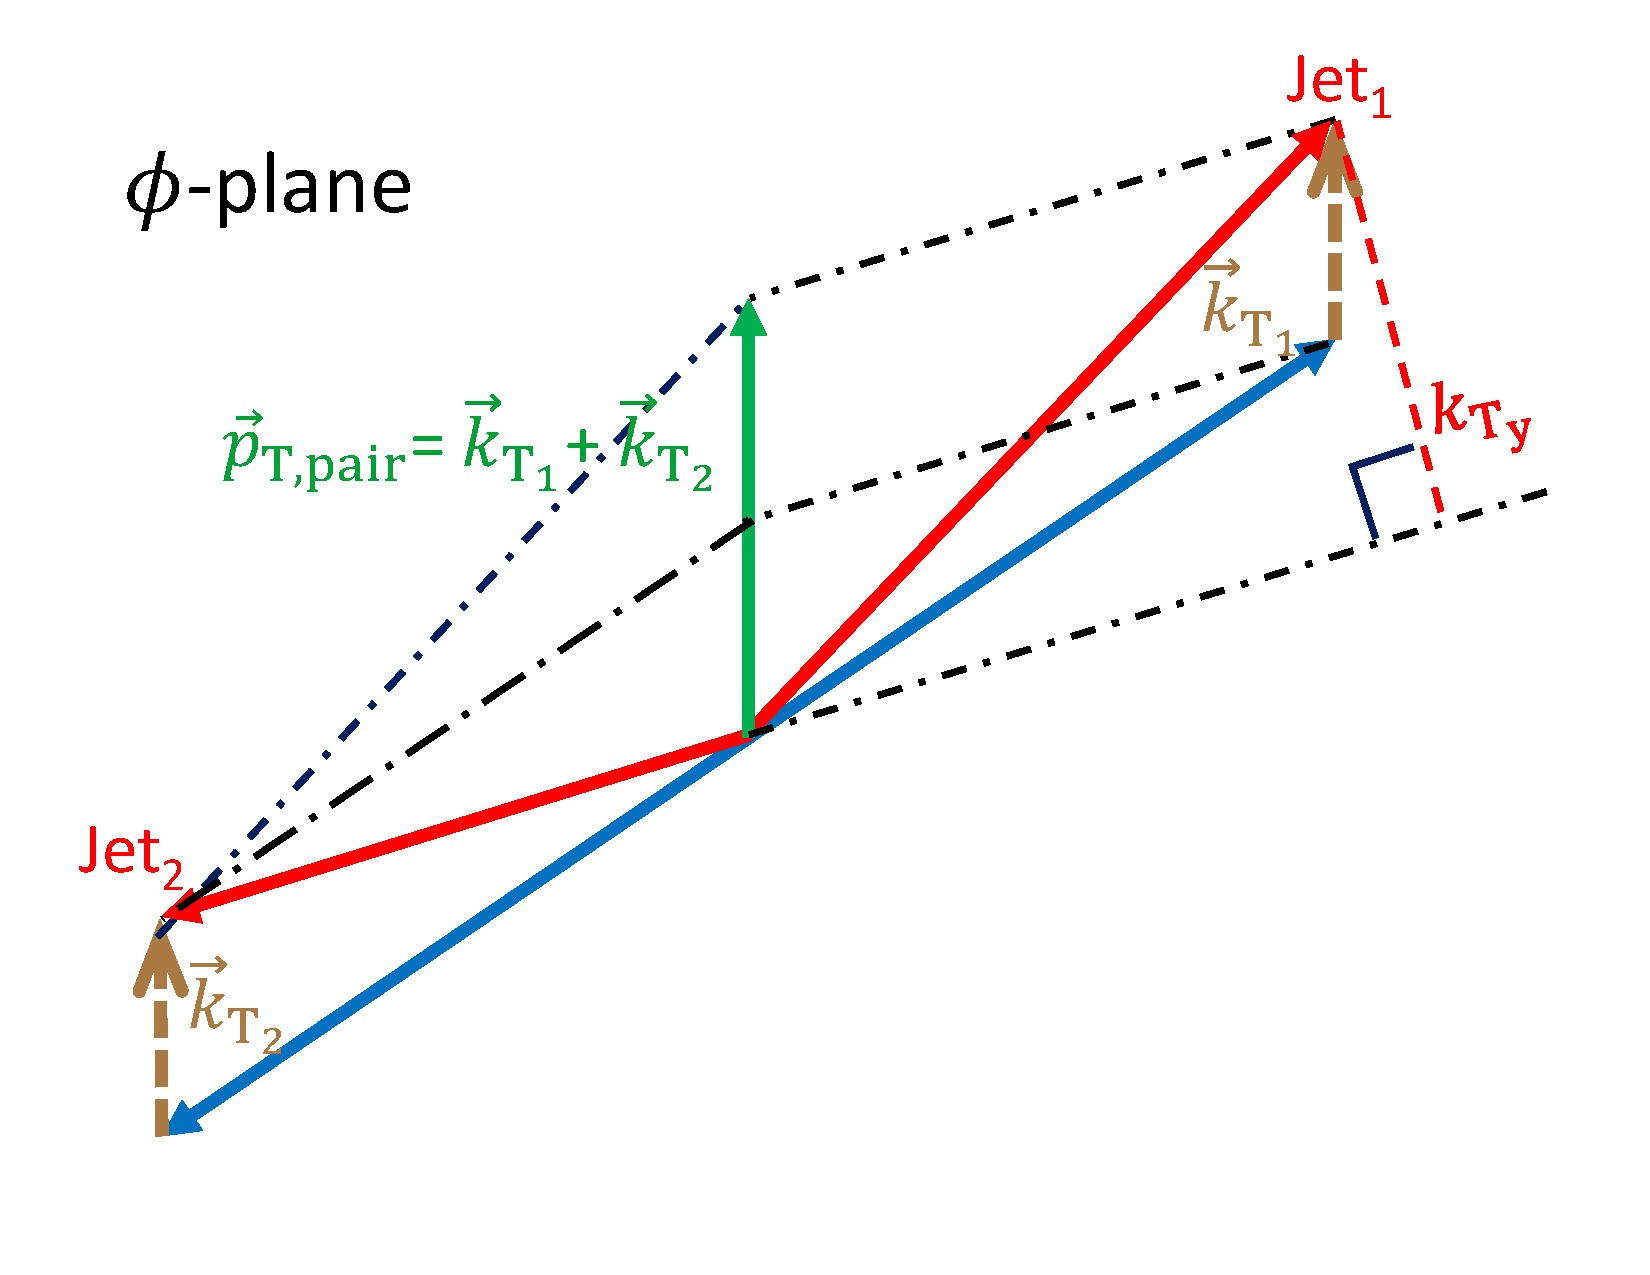
\includegraphics[width=1.0\textwidth]{kT_schematic}
\end{columns}
This topic
\begin{itemize}
	\item{Unbiased $p_\mathrm{T,pair}$ measurement with $\mathrm{{jet}_{leading}^{ch}}$ +  $\mathrm{{jet}_{sub-leading}^{ch}}$}
	\item{for Pb-Pb, p-Pb, pp and PYTHIA8}
\end{itemize}
\end{frame}

\begin{frame}
\frametitle{$\Delta \phi_\mathrm{dijet}$ for pp and p-Pb collisions}
\begin{columns}[t]
\column{.5\textwidth}
\centering
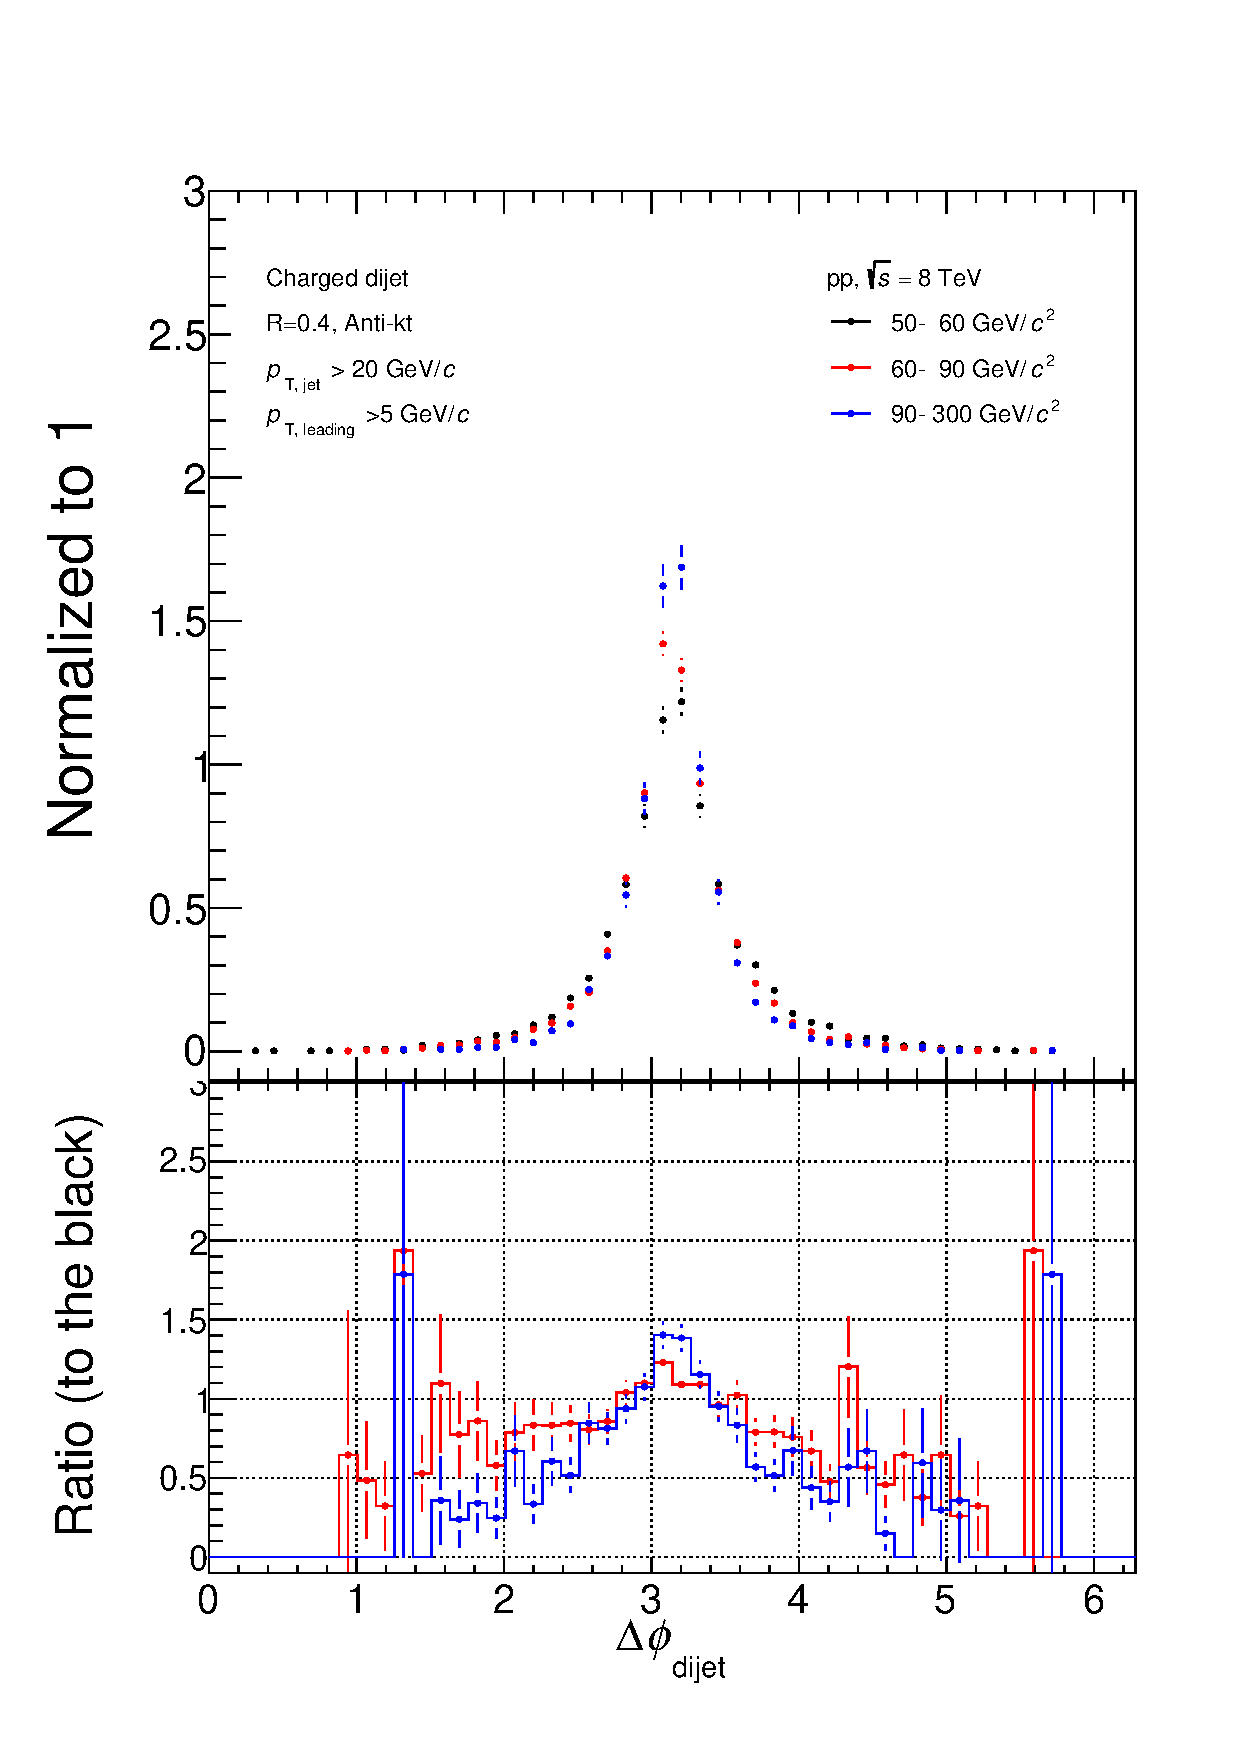
\includegraphics[width=1\linewidth]{dphi_pp_emcje}\\
\column{.5\textwidth}
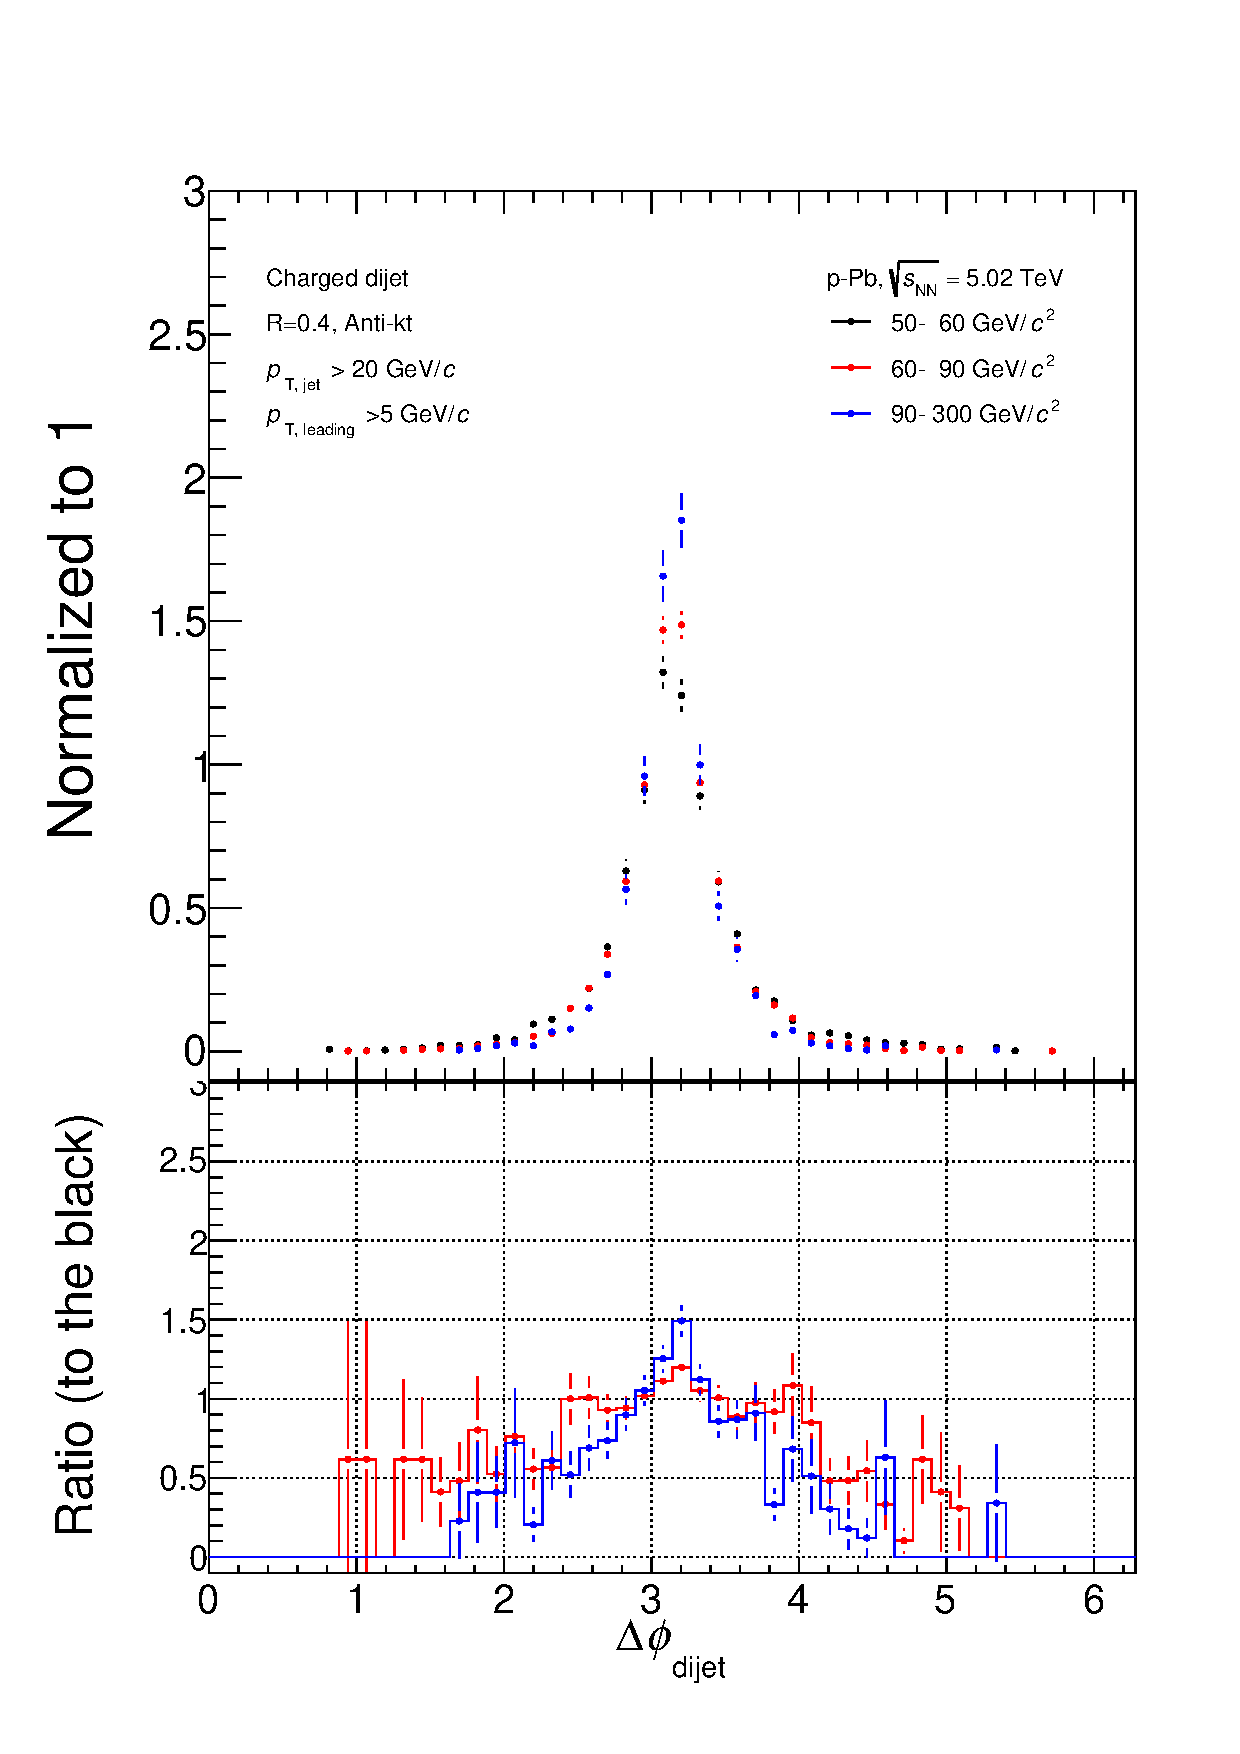
\includegraphics[width=1\linewidth]{dphi_ppb_emcje}\\
\end{columns}
\end{frame}

\begin{frame}

\frametitle{Unfolding}
Detector efficiency is corrected by multi-dimensional unfolding method
\begin{itemize}
\item{Package : RooUnfold}
\item{Algorithm : Iterative}
\end{itemize}

	\begin{equation}
	%\mathrm{Raw}(M_\mathrm{dijet},p_\mathrm{T,pair}) \times \frac{\mathrm{MC truth}(M_\mathrm{dijet},p_\mathrm{T,pair})}{\mathrm{MC rec}(M_\mathrm{dijet},p_\mathrm{T,pair})}
	(M_\mathrm{jj}^\mathrm{raw},p_\mathrm{T,jj}^\mathrm{raw}) \times \mathcal{R} (M_\mathrm{jj}^\mathrm{mcrec},M_\mathrm{jj}^\mathrm{mctrue},p_\mathrm{T,jj}^\mathrm{mcrec},p_\mathrm{T,jj}^\mathrm{mctrue})
	\end{equation}
Corrected $(M_\mathrm{jj}^\mathrm{corrected},p_\mathrm{T,jj}^\mathrm{corrected})$ 
\begin{itemize}
\item{projection on $M_\mathrm{jj}$ axis}
\item{projection on $p_\mathrm{T,jj}$ axis for different $M_\mathrm{jj}$ bin ranges}
\end{itemize}	

\end{frame}

\begin{frame}
\frametitle{Unfolding - closure test}
Closure test for the unfolding with MC samples
\begin{columns}[t]
\column{.5\textwidth}
\centering
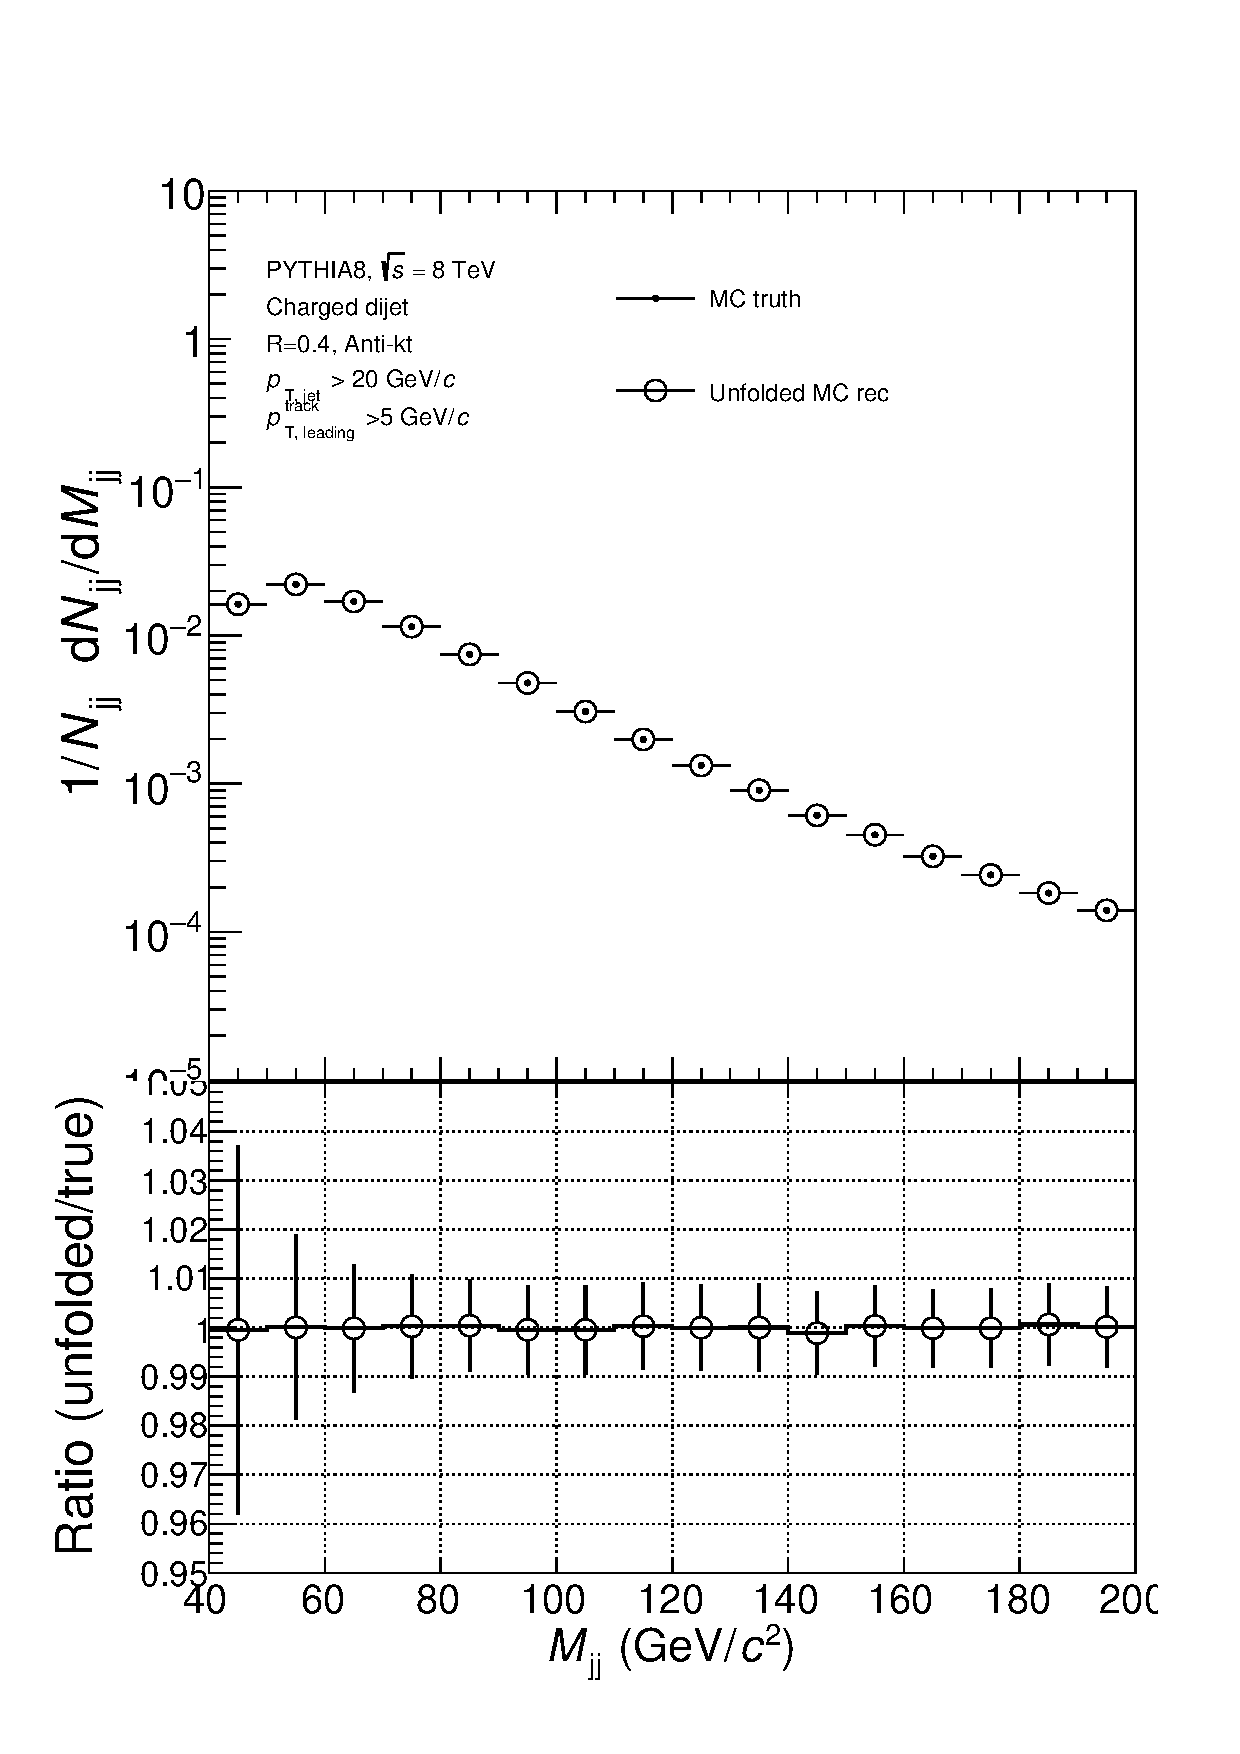
\includegraphics[width=1\linewidth]{mjj_closure}\\
\column{.5\textwidth}
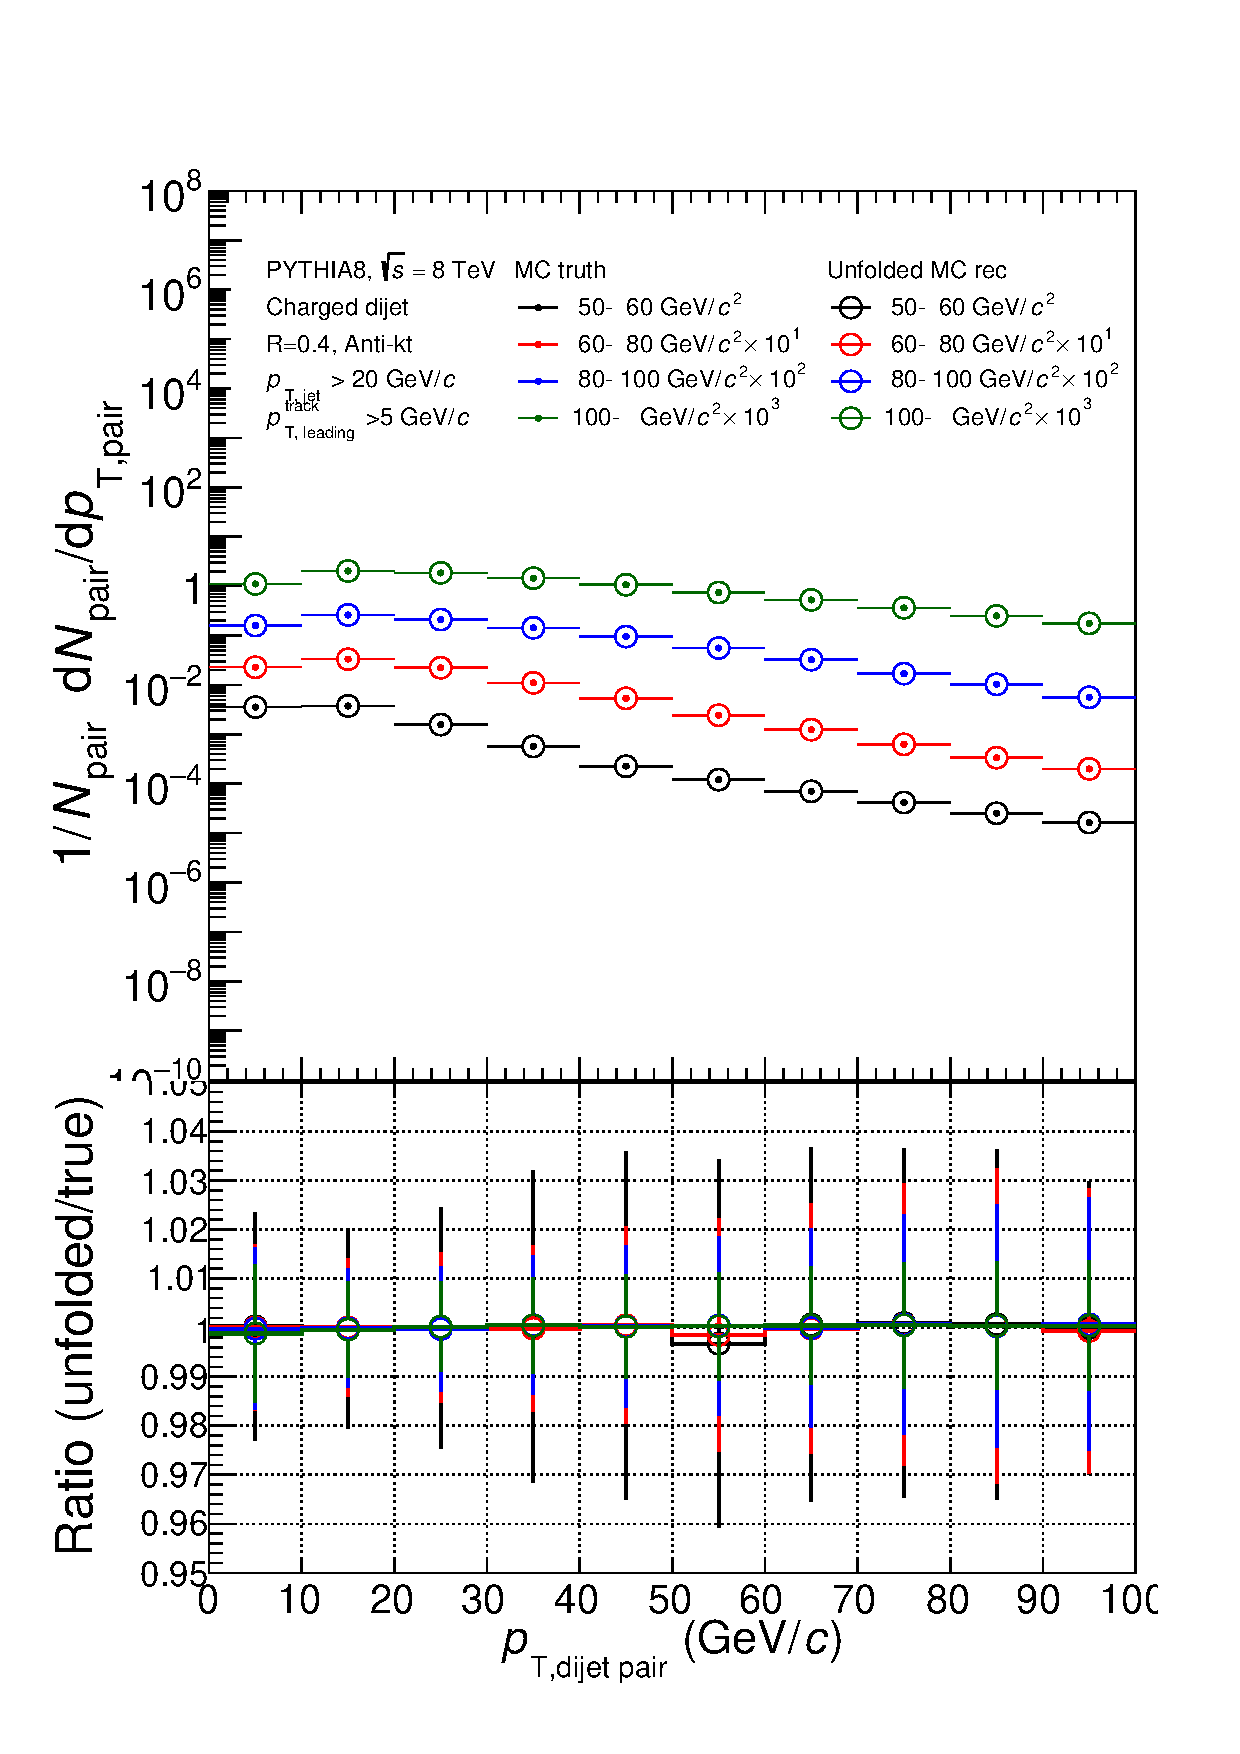
\includegraphics[width=1\linewidth]{ptjj_closure}\\
\end{columns}
\end{frame}


\begin{frame}
\frametitle{Charged dijet mass}
\begin{columns}[c]
\column{.5\textwidth}
\centering
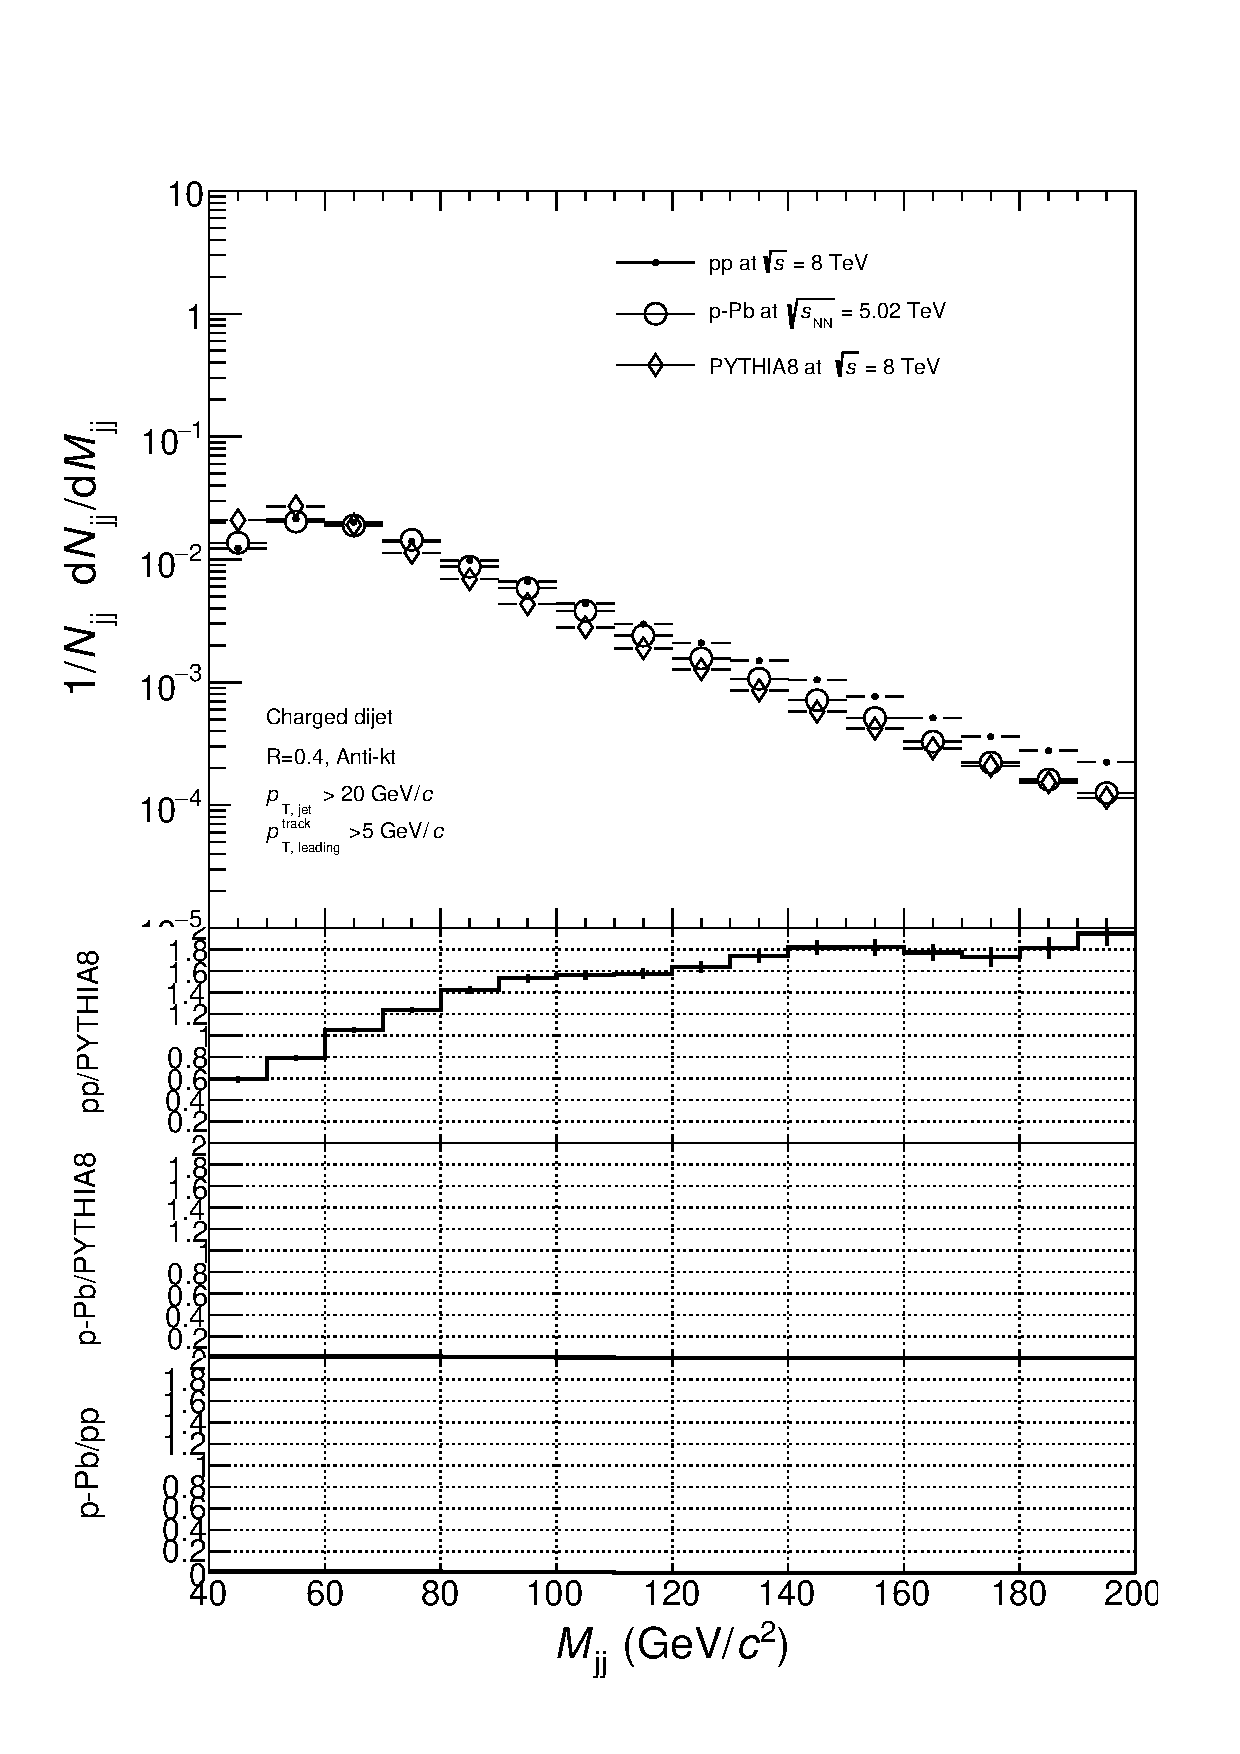
\includegraphics[width=1\linewidth]{../../Dijet/Figures/mjj_13d_pp_pPb}\\
\column{.5\textwidth}
Motivation\\
\begin{itemize}
	\item{To see medium effect of dijet invariant mass}
	\item{In medium, high virtuality \\ $\rightarrow$ Broad jet profile
	\\ $\rightarrow$ jet mass increases 
	\\ $\rightarrow$ dijet mass increases }
\end{itemize}

p-Pb v.s pp
\begin{itemize}
	\item{Finalizing study}
\end{itemize}
Pb-Pb v.s pp
\begin{itemize}
	\item{Study ongoing}
\end{itemize}

\end{columns}
\end{frame}




\begin{frame}
\frametitle{Charged dijet $k_\mathrm{T}$}
\begin{columns}[c]
\column{.5\textwidth}
\centering
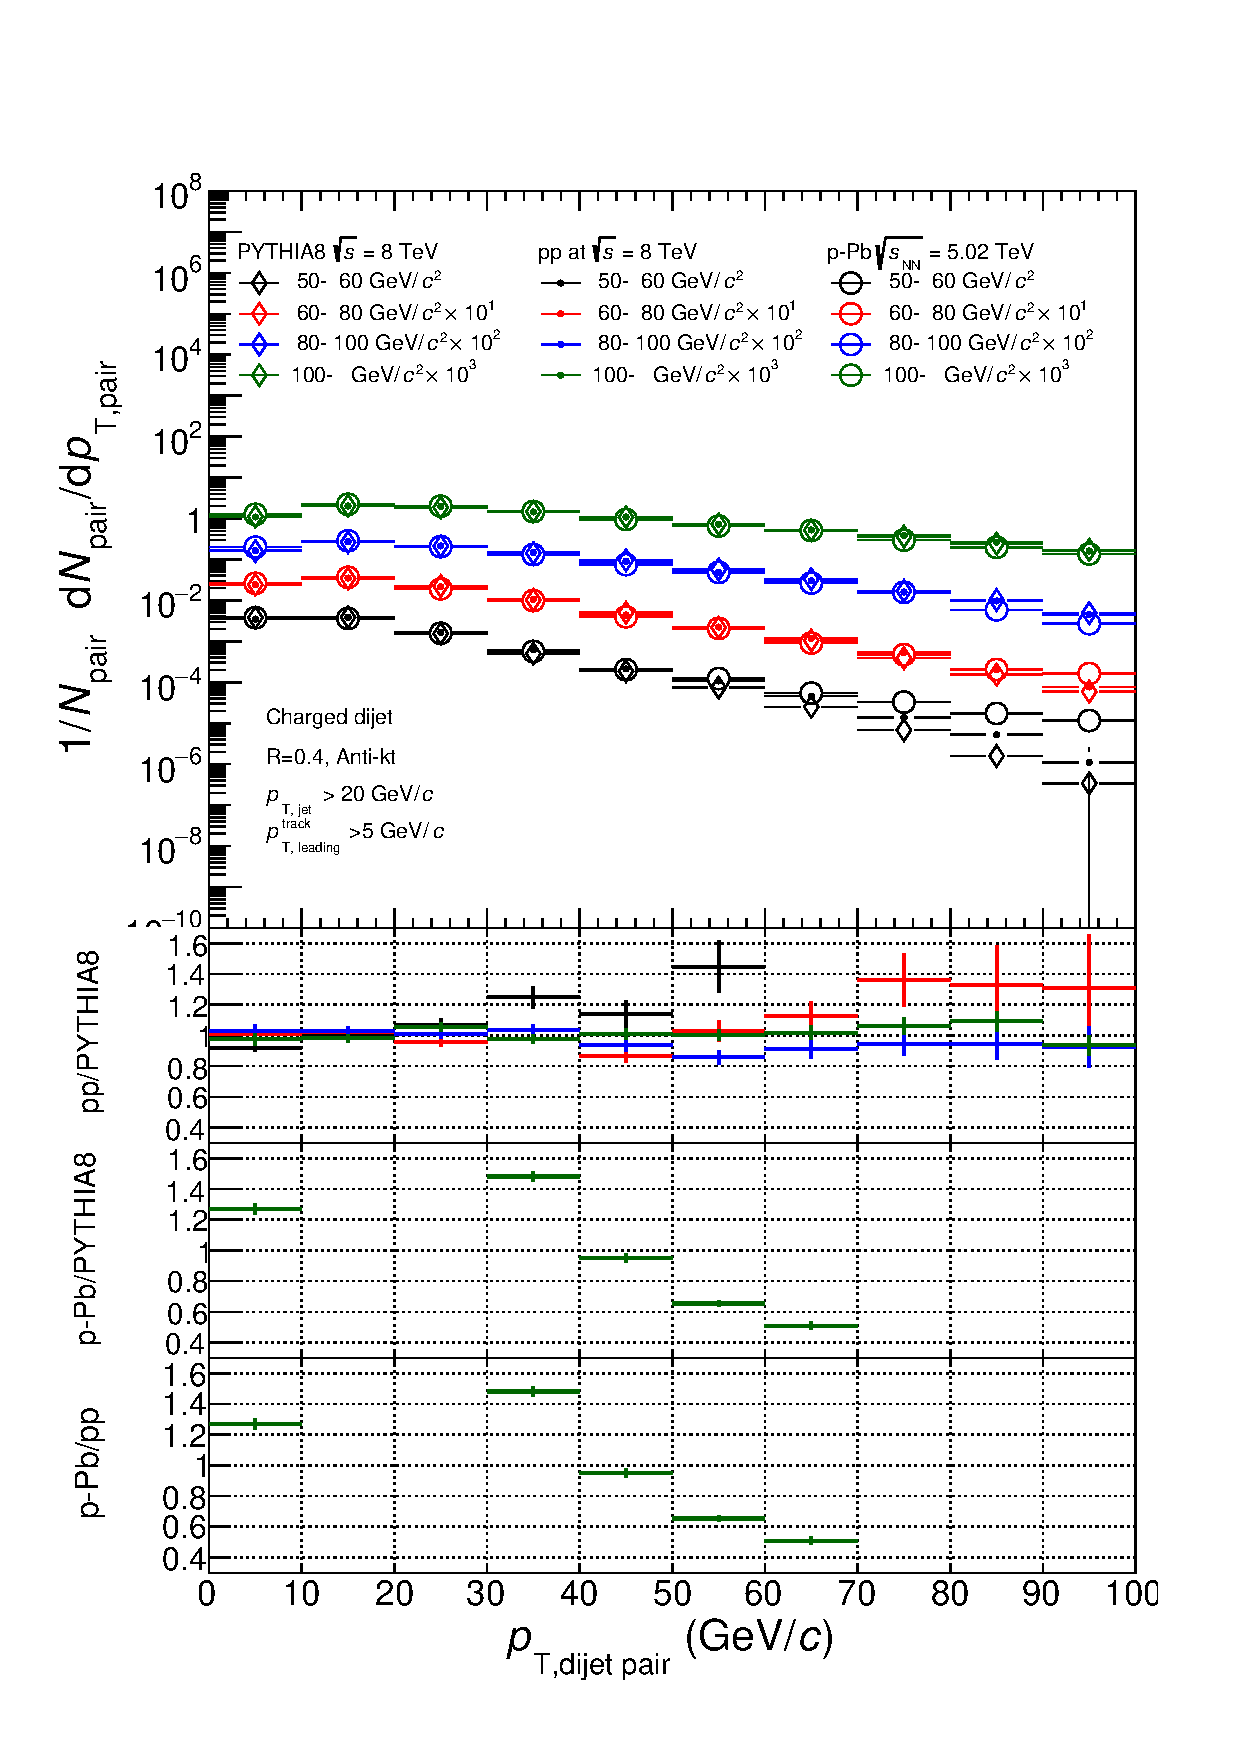
\includegraphics[width=1\linewidth]{../../Dijet/Figures/ptjj_13d_pp_pPb}\\
\column{.5\textwidth}
Motivation\\
\begin{itemize}
	\item{To see medium effect of dijet acoplanarity}
	\item{In medium, dijet imbalance increases (increasing  $k_\mathrm{T}$)}
\end{itemize}

p-Pb v.s pp
\begin{itemize}
	\item{Finalizing study}
\end{itemize}
Pb-Pb v.s pp
\begin{itemize}
	\item{Study ongoing}
\end{itemize}

\end{columns}
\end{frame}



\begin{frame}
\frametitle{Pb-Pb at $\sqrt{s}$ = 5.02 TeV}
\begin{itemize}
\item Data : LHC15o
\item Trigger selection : INT7
\item $\#$ of events scanned : 17 millions 
\item Underlying events have to be subtracted
\end{itemize}
\end{frame}

\begin{frame}
\frametitle{Correction for the underlying event}
In Pb-Pb, bkg from underlying events is considered!\\
\begin{itemize}
	\item{Bkg densities are measured with $\mathrm{kT}$ cones by median}
		\begin{itemize}
			\item{$p_\mathrm{T,patch}$ = $\sum_{i \in \mathrm{patch}} p_\mathrm{T,i}$, $m_{\delta,patch} = \sum_{i \in \mathrm{patch}} (\sqrt{m_i^2+p_\mathrm{T,i}^2} - p_\mathrm{T,i})$}
			\item{$\rho$=$\mathrm{median}_\mathrm{patches}$ $\{ \frac{p_\mathrm{T,patch}}{A_\mathrm{patch}}\}$, $\rho_m$=$\mathrm{median}_\mathrm{patches}$ $\{ \frac{m_\mathrm{\delta,patch}}{A_\mathrm{patch}}\}$}
		\end{itemize}
	\item{anti-$\mathrm{kT}$ jets are recalculated by this bkg density with $\mathrm{kT}$ cones }
	\begin{itemize}
		\item $p^{\mu}_\mathrm{corr} = (p^x-\rho A^x, p^y-\rho A^y, p^z-(\rho+\rho_m)A^z, E-(\rho+\rho_m)A^E)$
	\end{itemize}
\end{itemize}

\end{frame}

\begin{frame}
\frametitle{Inclusive $p_\mathrm{T,jet}$ before and after the correction}
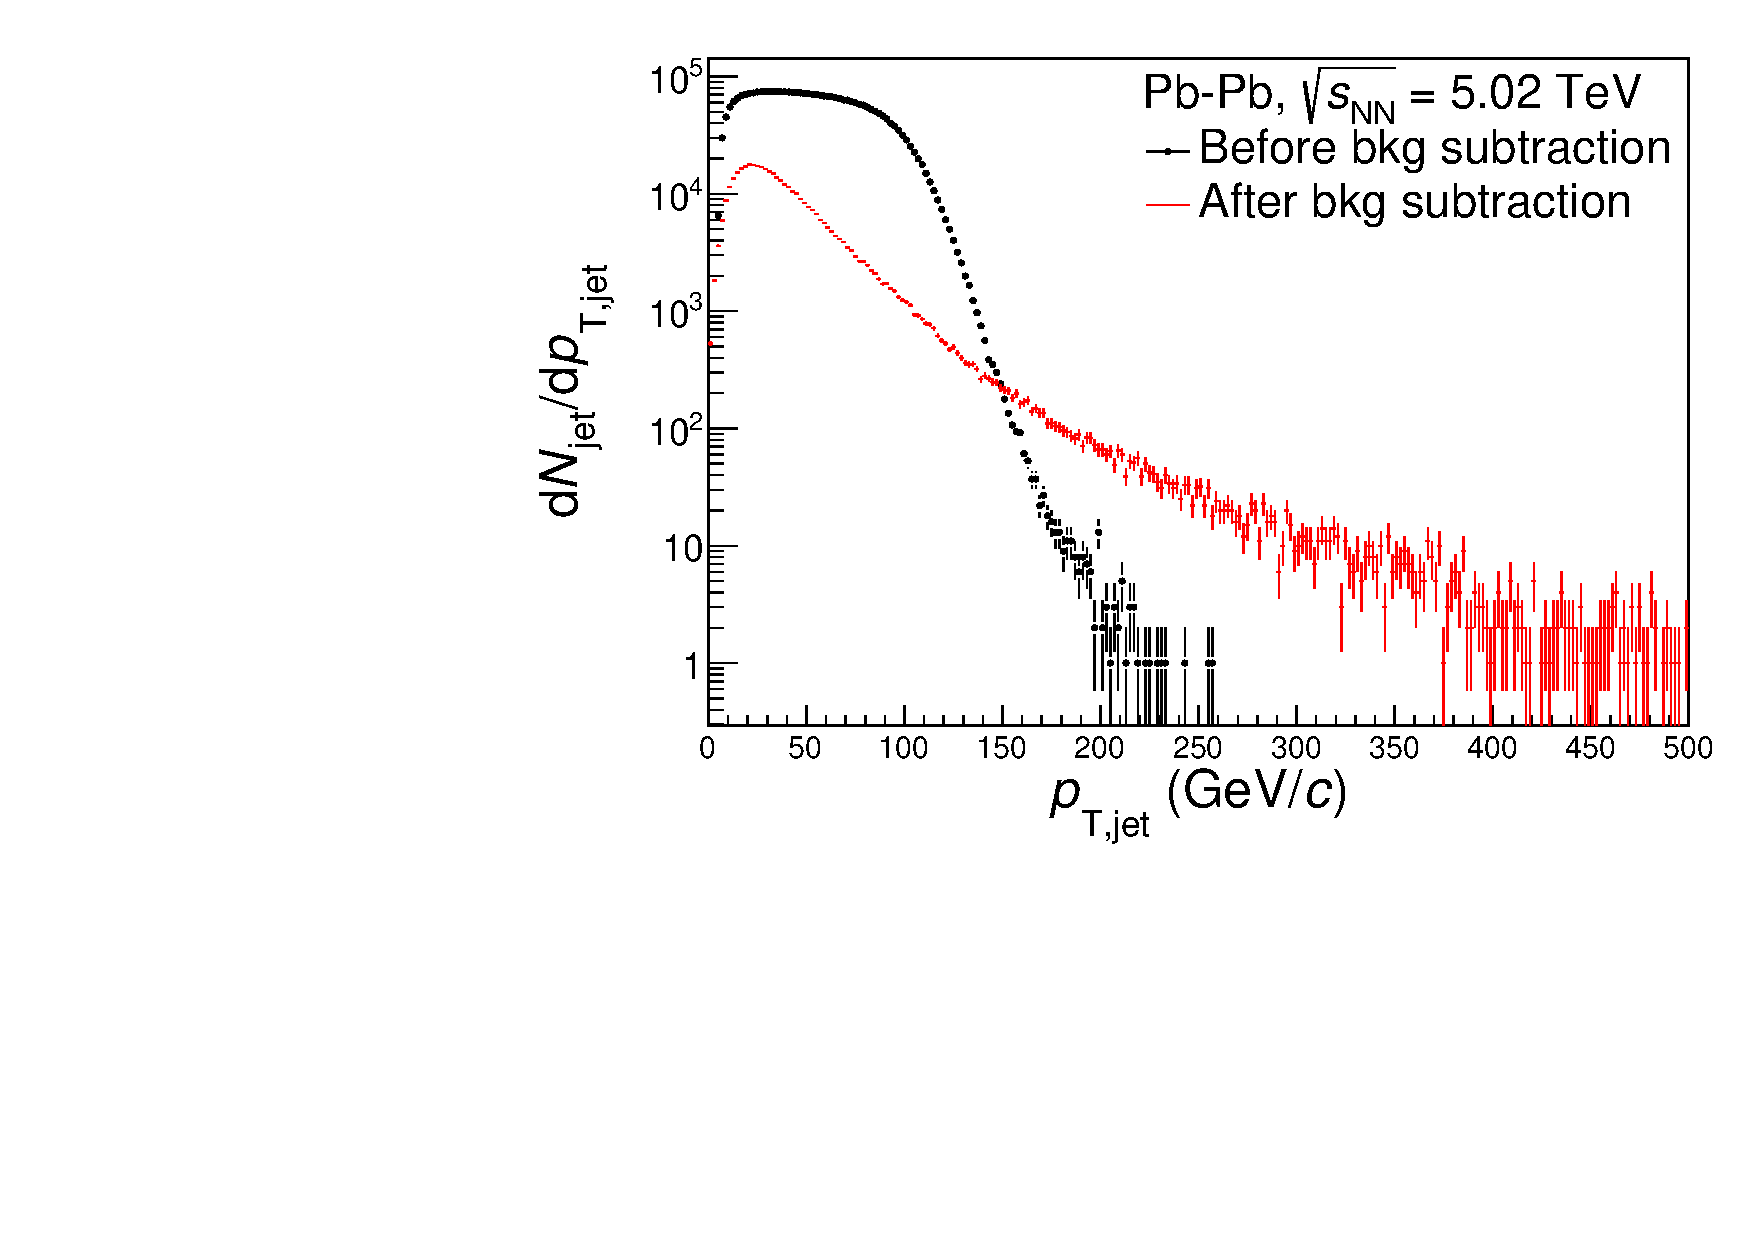
\includegraphics[width=1\linewidth]{JetPtBAcorrection}\\
\end{frame}

\begin{frame}
\frametitle{Inclusive jet mass before and after the correction}
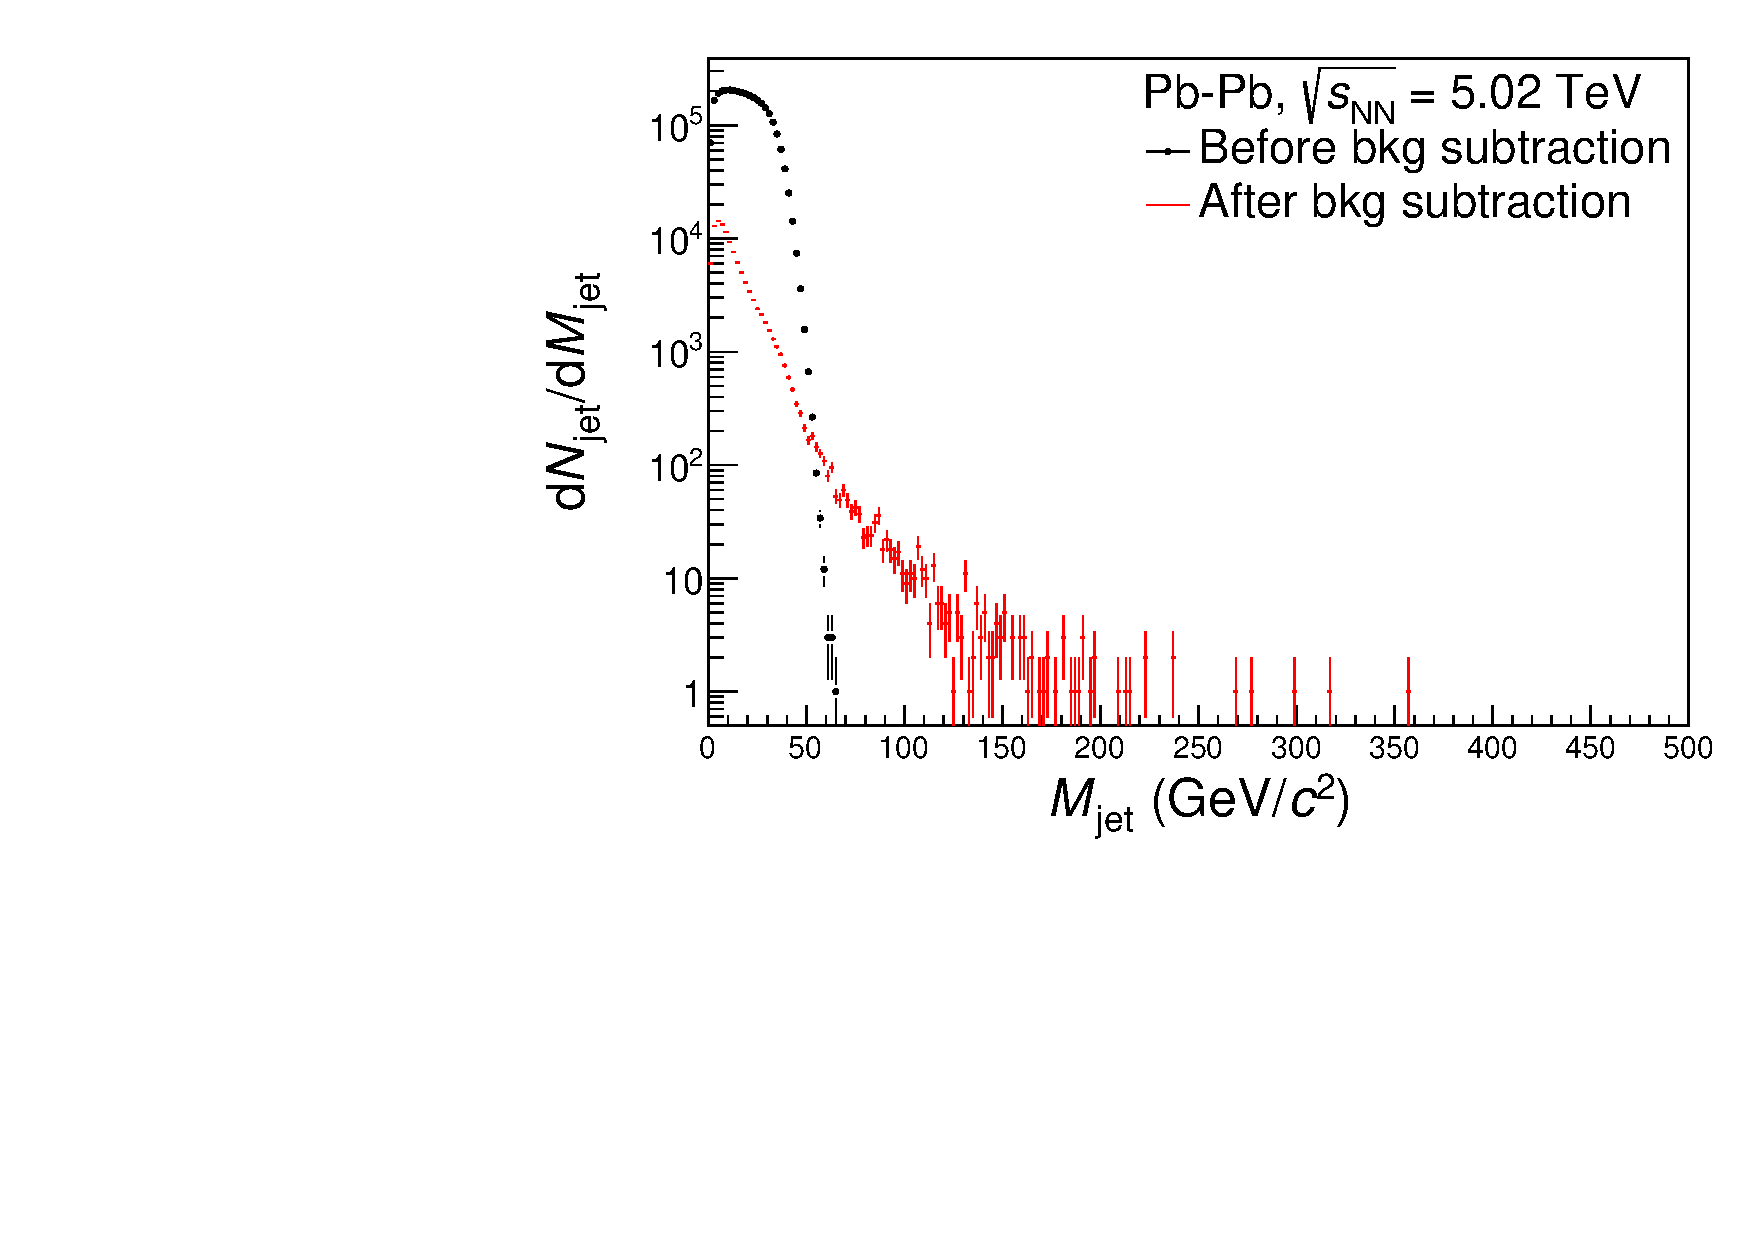
\includegraphics[width=1\linewidth]{JetMassBACorrection}\\
\end{frame}

\begin{frame}
\frametitle{$\Delta \phi_\mathrm{dijet}$ for Pb-Pb collisions}
\begin{columns}[c]
\column{.5\textwidth}
\centering
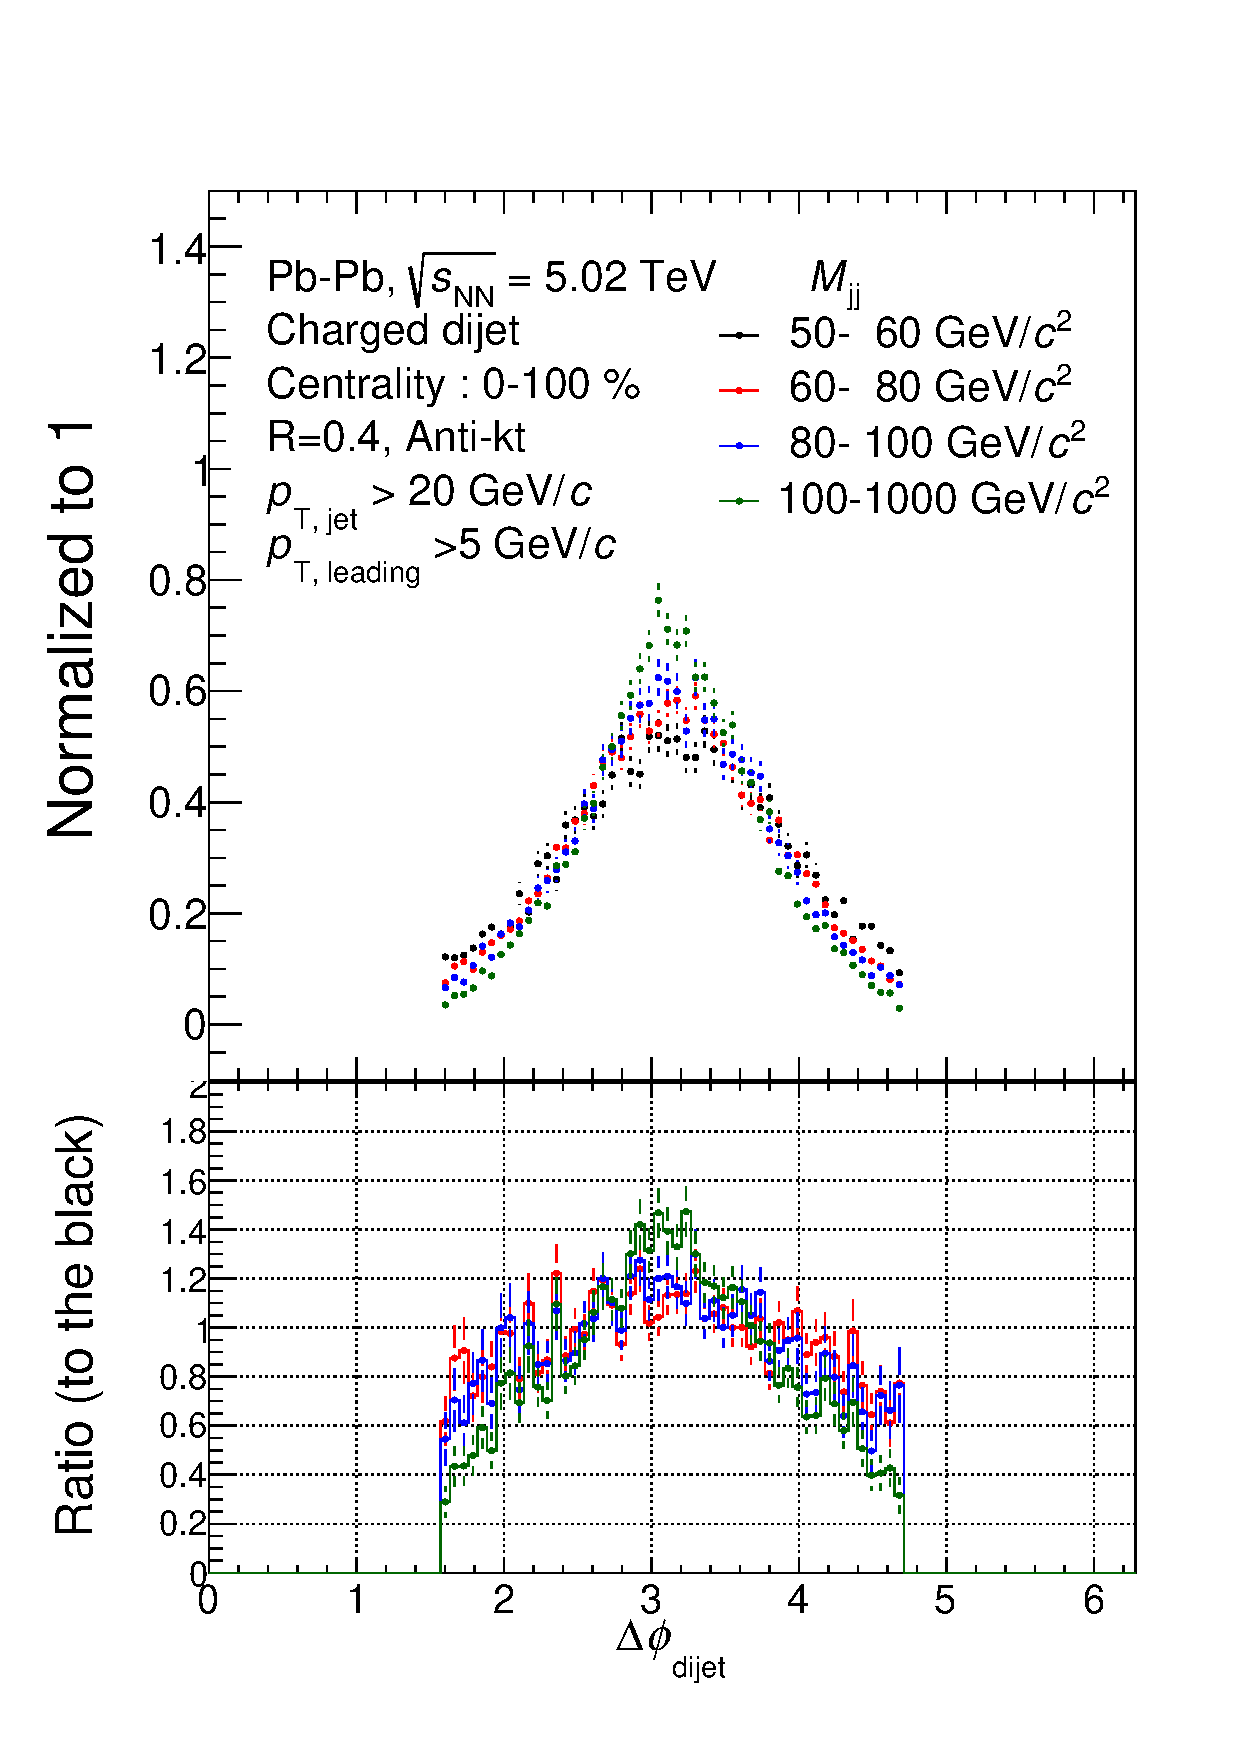
\includegraphics[width=1\linewidth]{PbPb_dphi_0_100}\\
\column{.5\textwidth}
\begin{itemize}
\item Bugs were fixed
\item 14 millions MB events scanned
\item $\Delta \phi$ dist. show good shapes
\end{itemize}
\end{columns}
\end{frame}

\begin{frame}
\frametitle{Raw $M_\mathrm{jj}$ for Pb-Pb collisions}
\begin{columns}[c]
\column{.5\textwidth}
\centering
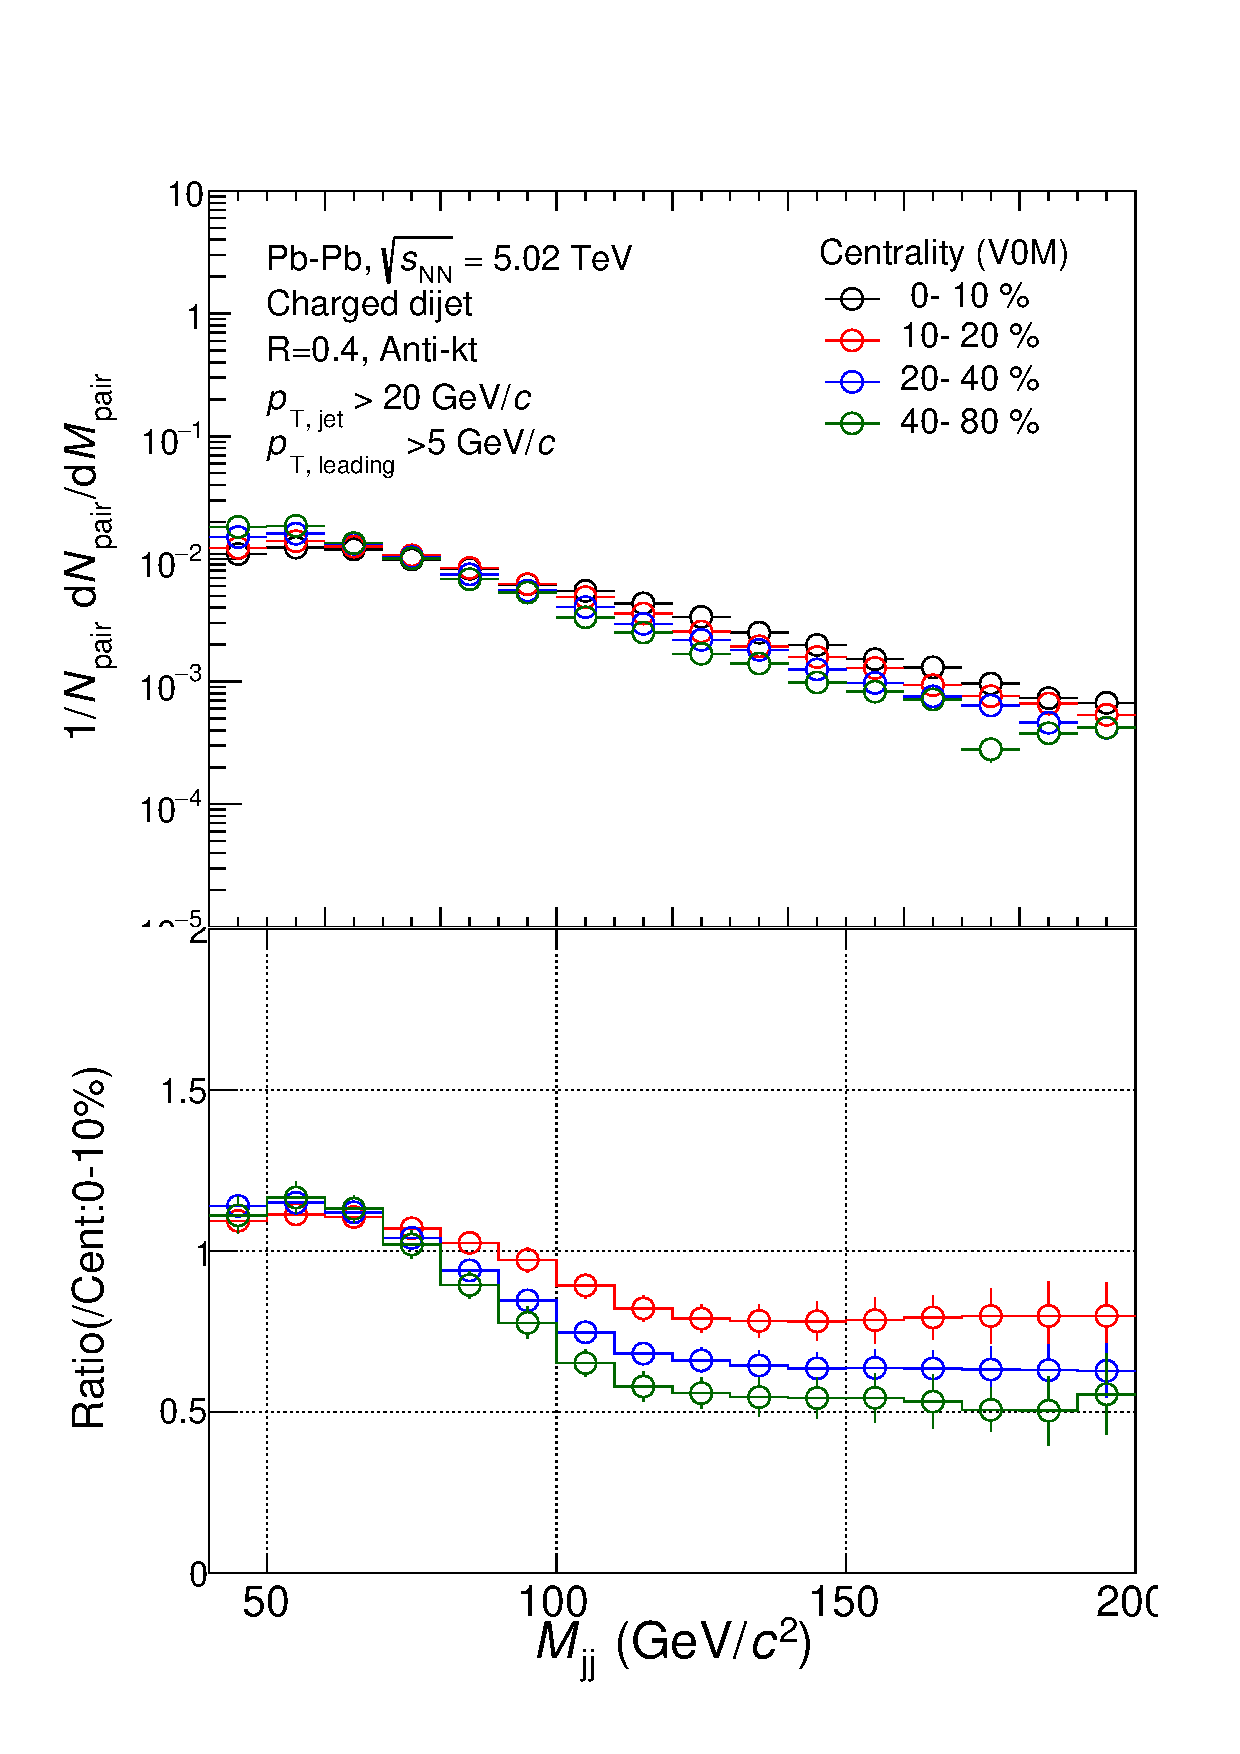
\includegraphics[width=1\linewidth]{PbPb_mjj}\\
\column{.5\textwidth}
\begin{itemize}
\item More central $\rightarrow$ higher dijet mass
\end{itemize}
\end{columns}
\end{frame}

\begin{frame}
\frametitle{Raw $p_\mathrm{T,pair}$ for Pb-Pb collisions}
\begin{columns}[c]
\column{.5\textwidth}
\centering
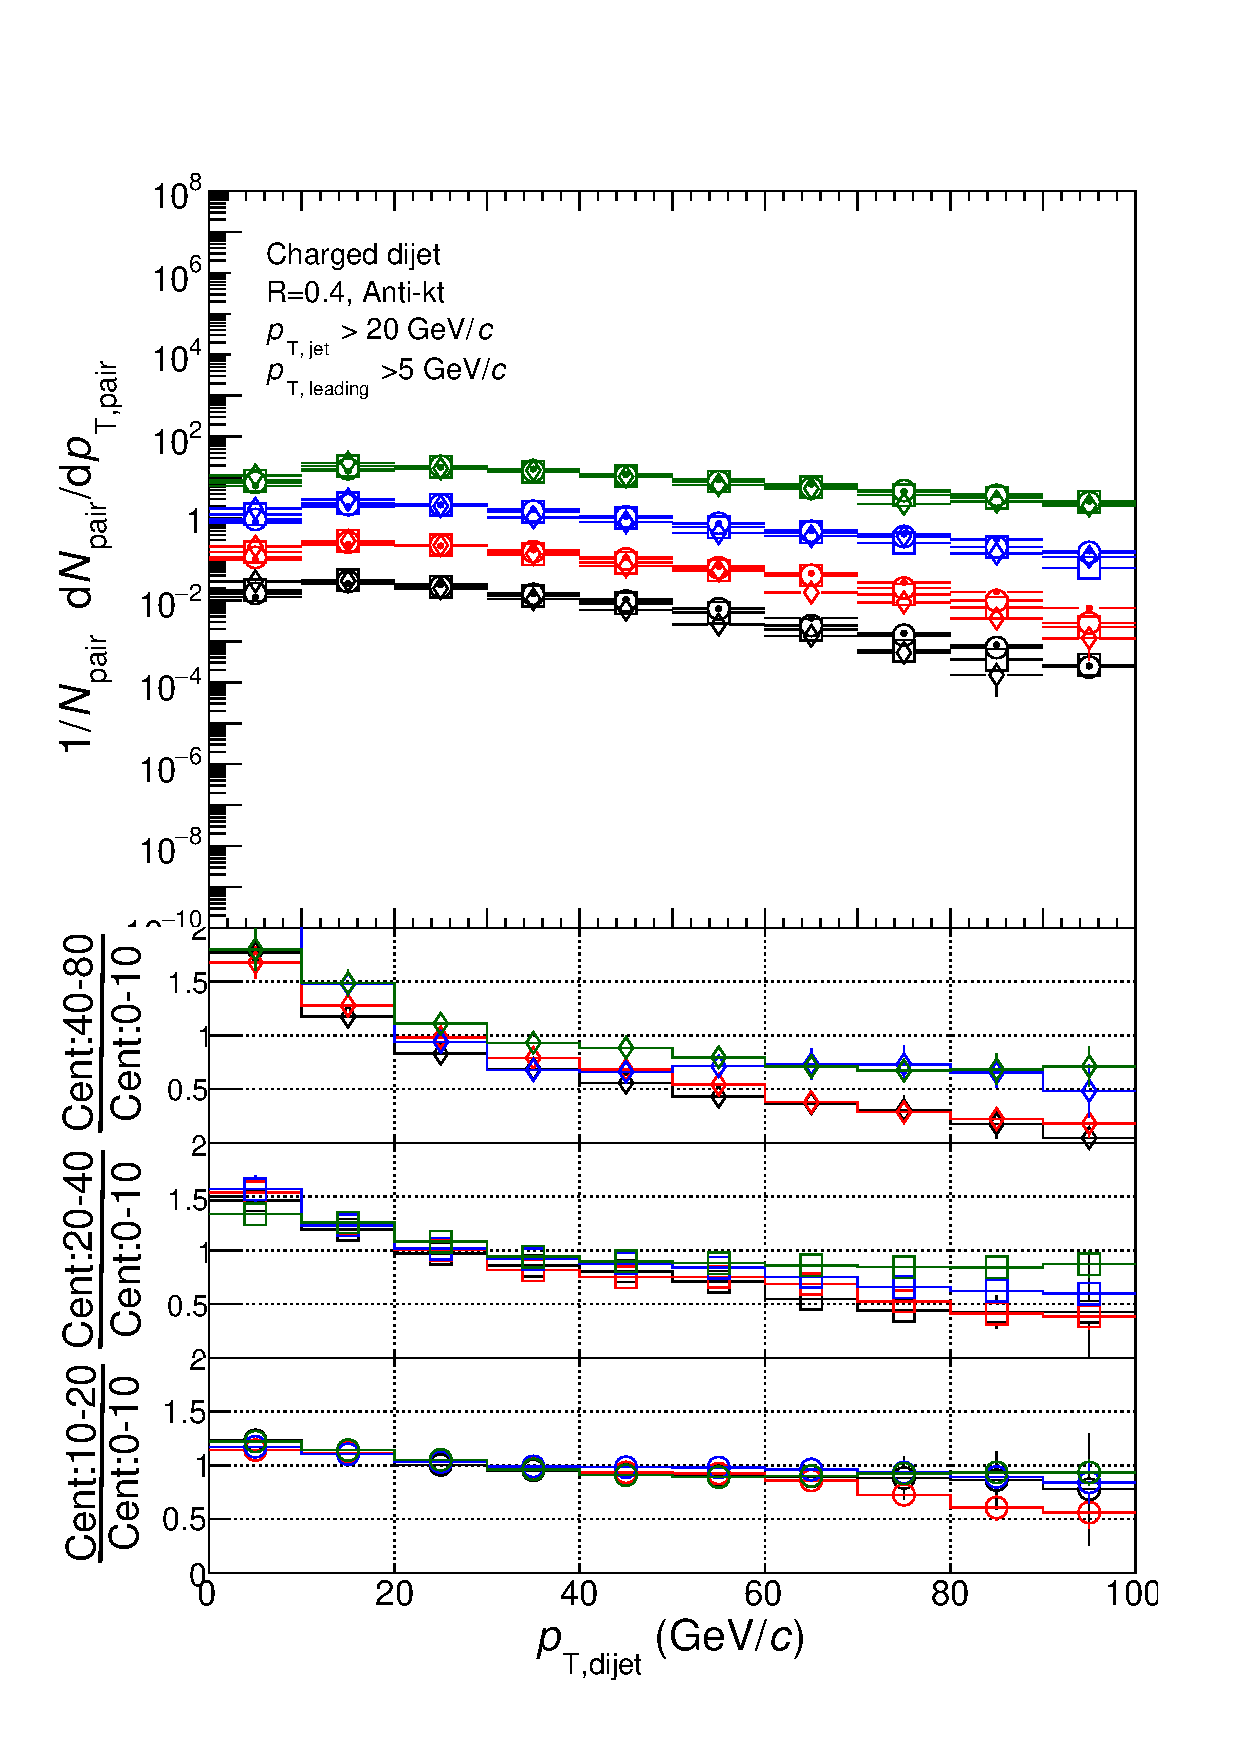
\includegraphics[width=1\linewidth]{PbPb_ptpair}\\
\column{.5\textwidth}
\begin{itemize}
\item More central $\rightarrow$ higher $p_\mathrm{T,pair}$
\end{itemize}
\end{columns}
\end{frame}


